\section{Shepherding Process}
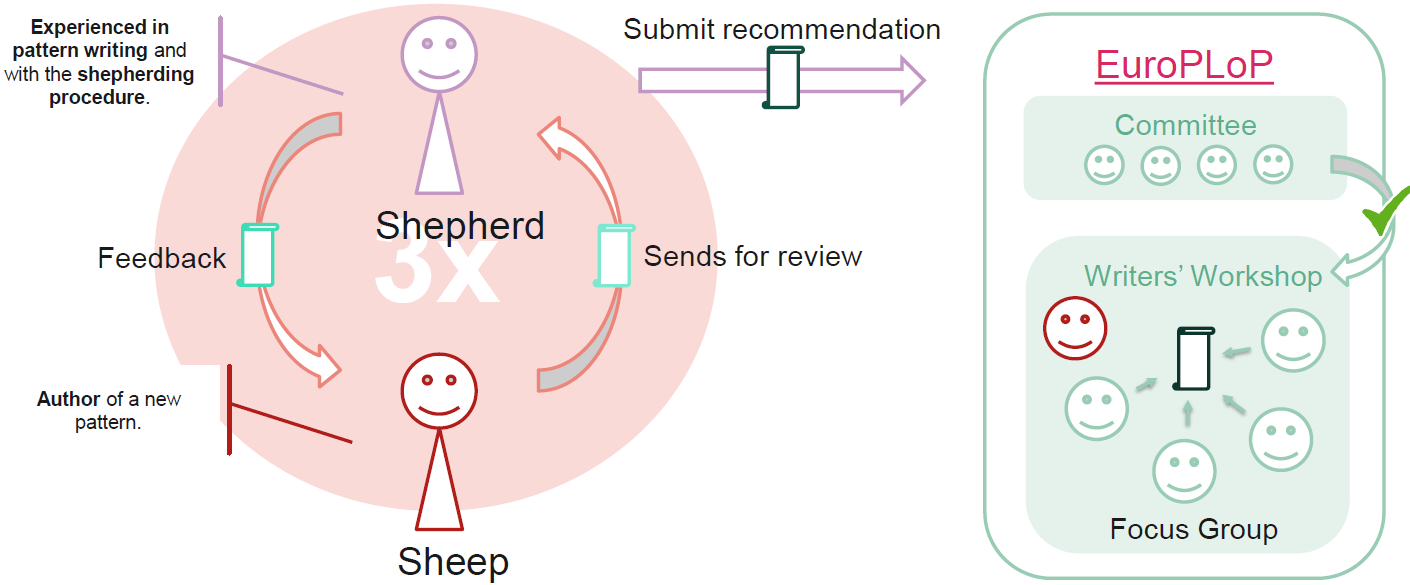
\includegraphics[width=\linewidth]{shepherding.png}
\subsection{Process}
\textbf{1. Three Iterations}
\begin{itemize}
    \item How to budget your time and effort to make shepherding effective
\end{itemize}
\textbf{2. The Shepheade Know the Sheep}
\begin{itemize}
    \item How to establish a productive relationship between you and the author
\end{itemize}
\textbf{3. Half a Loaf}
\begin{itemize}
    \item How to make sure that shepheadring continous to move forward
\end{itemize}
\textbf{4. Big Picture}
\begin{itemize}
    \item How to gasp the gist of the pattern right off the bat
\end{itemize}
\textbf{5. Author as Owner}
\begin{itemize}
    \item How to keep from writing the pattern for the author
\end{itemize}
\textbf{6. Forces Define Problem}
\begin{itemize}
    \item How to understand the problem at a deeper level
\end{itemize}

\subsection{Writer's Workshop}
\begin{itemize}
    \item Used to improve patterns
    \item Primary focus of PLoP (PATTERN LANGUAGES OF PROGRAMS)
    \item The authors of the paper under discussion remain silent
    \item Major target: Get a lot of feedback and suggestions
\end{itemize}
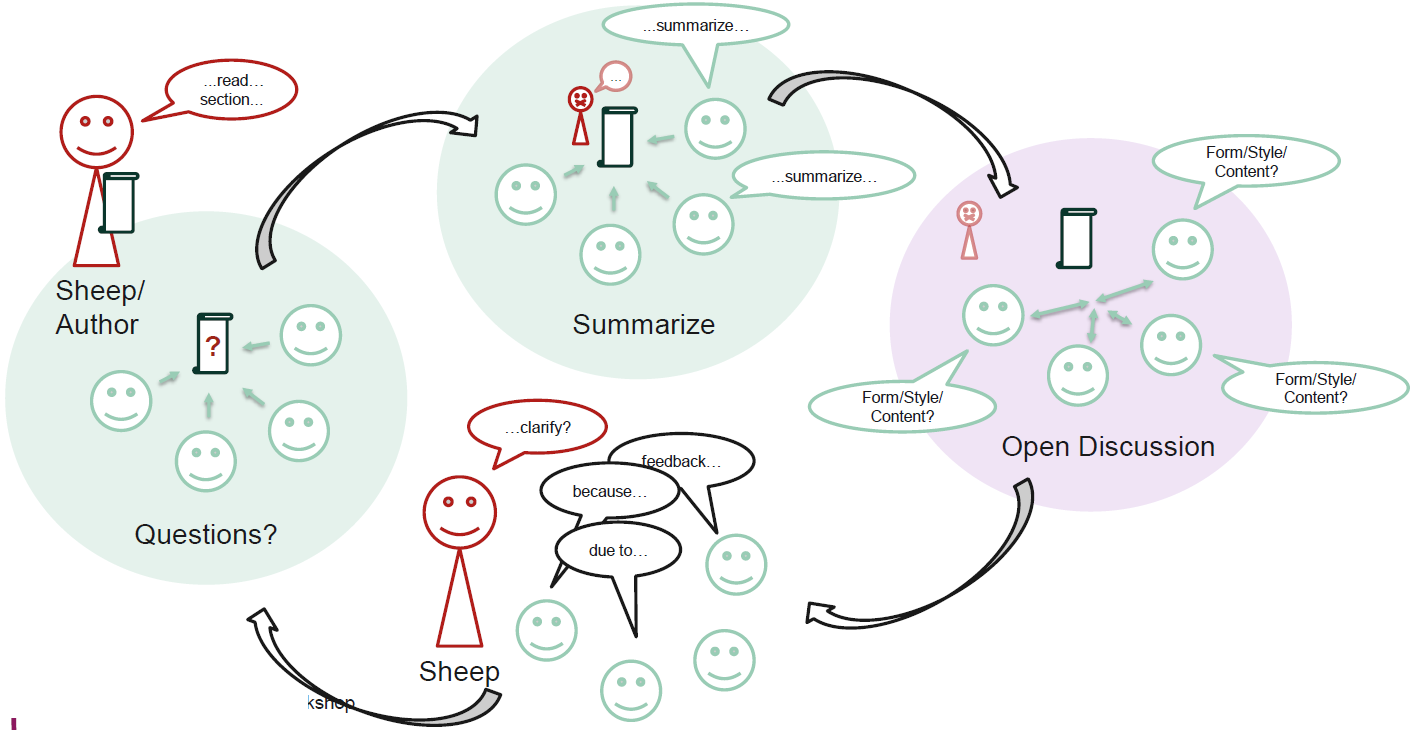
\includegraphics[width=\linewidth]{writers_workshop.png}

\subsubsection{1) Pattern Scanning}
Does reading the pattern problem, solution, known uses, context, forces, consequences make sense?

\subsubsection{2) Styling the Forces}
Are forces listed as items?

\subsubsection{3) BUT Style}
\begin{itemize}
    \item Is BUT-Style used and does it build tension?
    \item Does it lead to bold face solution?
\end{itemize}

\subsubsection{4) Detailed Example / Technical Diagram}
Is there a detailed example and technical diagram?

\subsubsection{5) Known Uses}
Are there at least three know and approprate uses

\subsubsection{6) Relationship}
\begin{itemize}
    \item Are the related patterns described in a logical order?
    \item Are the relationships appropriate?
\end{itemize}

\subsubsection{7) Sstand-Alone, Self-Contained}
\begin{itemize}
    \item Does the pattern overlap with other patterns?
    \item Is the pattern description coherent?
    \item Are there suggestions for improvement?
\end{itemize}
